\documentclass[letterpaper,12pt]{article}
\usepackage[section=2.5]{mathhw}

\usepackage{tikz}
\definecolor{bookblue}{RGB}{0, 173, 239}
\definecolor{bookgrey}{RGB}{219, 220, 222}

\begin{document}

\maketitle

\begin{enumerate}
  \item[71.]
    An oil exploration company currently has two active projects, one in Asia and the other in Europe. Let $A$ be the event that the Asian project is successful and $B$ be the event that the European project is successful. Suppose that $A$ and $B$ are independent events with $P(A) = .4$ and $P(B) = .7$.
    \begin{enumerate}
      \item[a.]
        If the Asian project is not successful, what is the probability that the European project is also not successful? Explain your reasoning.
        \begin{align*}
          P(B^\prime|A^\prime) = P(B^\prime) = 1 - P(B) = 1 - .7 = .3
        \end{align*}
        $A$ and $B$ are independent, so their complements are also independent. Furthermore, this means the occurrence of $A^\prime$ does not affect the probability of $B^\prime$. Thus, it can be simplified to $P(B^\prime)$.
      \item[b.]
        What is the probability that at least one of the two projects will be successful?
        \begin{align*}
          P(A \cup B) &= P(A) + P(B) - P(A \cap B) \\
          &= P(A) + P(B) - (P(A) \cdot P(B)) \\
          &= .4 + .7 - (.4 \times .7) \\
          &= .82
        \end{align*}
      \item[c.]
        Given that at least one of the two projects is successful, what is the probability that only the Asian project is successful?
        \begin{align*}
          P((A \cap B^\prime)|(A \cup B)) &= \frac{P((A \cap B^\prime) \cap (A \cup B))}{P(A \cup B)}
        \end{align*}
        The commutative, associative, and absorption laws can be used to simplify the numerator.
        \begin{align*}
          (A \cap B^\prime) \cap (A \cup B) &= (B^\prime \cap A) \cap (A \cup B) \\
          &= B^\prime \cap (A \cap (A \cup B)) \\
          &= B^\prime \cap A
        \end{align*}
        Since the events are independent, this enables the numerator to be calculated using the multiplication rule.
        \begin{align*}
          P((A \cap B^\prime)|(A \cup B)) &= \frac{P(B^\prime \cap A)}{P(A \cup B)} \\
          &= \frac{P(B^\prime) \cdot P(A)}{P(A \cup B)} \\
          &= \frac{.3 \times .4}{.82} \\
          &\approx .146
        \end{align*}
    \end{enumerate}
  \item[74.]
    The proportions of blood phenotypes in the U.S. population are as follows:
    \begin{center}
      \begin{tabular}{cccc}
        A & B & AB & O \\
        .40 & .11 & .04 & .45
      \end{tabular}
    \end{center}
    Assuming that the phenotypes of two randomly selected individuals are independent of one another, what is the probability that both phenotypes are O? What is the probability that the phenotypes of two randomly selected individuals match?
    \begin{align*}
      P(O \cap O) = P(O) \cdot P(O) = {.45}^2 = .2025
    \end{align*}
    The events that both individuals have a specific phenotype are disjoint since each individual can only have one phenotype. Hence, the unions below can be decomposed into a simple sum, without having to account for any intersections.
    \begin{align*}
      &P((A \cap A) \cup (B \cap B) \cup (AB \cap AB) \cup (O \cap O)) \\
      &= P(A \cap A) + P(B \cap B) + P(AB \cap AB) + P(O \cap O) \\
      &= P(A)^2 + P(B)^2 + P(AB)^2 + P(O)^2 \\
      &= {.40}^2 + {.11}^2 + {.04}^2 + {.45}^2 \\
      &= .16 + .0121 + .0016 + .2025 \\
      &= .3762
    \end{align*}
  \item[77.]
    An aircraft seam requires 25 rivets. The seam will have to be reworked if any of these rivets is defective. Suppose rivets are defective independently of one another, each with the same probability.
    \\ \\
    Let $A$ be the event that a seam is good. Let $B$ be the event that a rivet is good.
    \begin{enumerate}
      \item[a.]
        If 15\% of all seams need reworking, what is the probability that a rivet is defective?
        \begin{align*}
          P(A) &= P(B_1 \cap B_2 \ldots \cap B_{25}) = P(B)^{25}
        \end{align*}
        \begin{align*}
          P(A^\prime) &= 1 - P(A) \\
          .15 &= 1 - P(B)^{25} \\
          P(B)^{25} &= 1 - .15 \\
          P(B) &= \sqrt[25]{.85} \\
          &\approx .9935203
        \end{align*}
        \begin{align*}
          P(B^\prime) = 1 - P(B) \approx 1 - .9935203 \approx .0064797
        \end{align*}
      \item[b.]
        How small should the probability of a defective rivet be to ensure that only 10\% of all seams need reworking?
        \begin{align*}
          P(B^\prime) &= 1 - \sqrt[25]{1 - .10} \\
          &\approx .0042056
        \end{align*}
    \end{enumerate}
  \item[80.]
    Consider the system of components connected as in the accompanying picture. Components 1 and 2 are connected in parallel, so that subsystem works iff either 1 or 2 works; since 3 and 4 are connected in series, that subsystem works iff both 3 and 4 work. If components work independently of one another and $P$(component $i$ works) $= .9$ for $i = 1,2$ and $= .8$ for $i = 3,4$, calculate $P$(system works).
    \begin{center}
      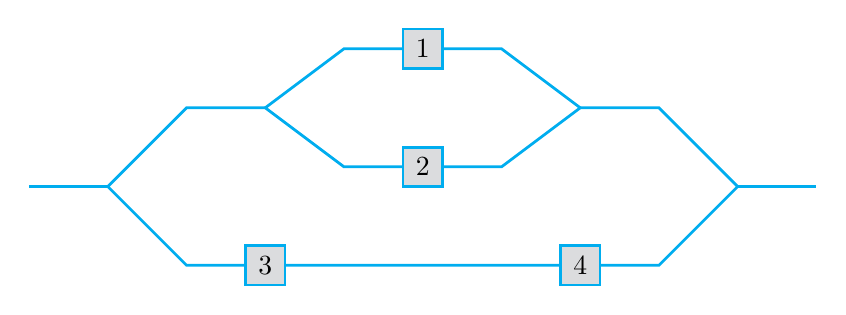
\begin{tikzpicture}[line width=1pt, draw=bookblue]
        \coordinate (A1) at (1,0);
        \coordinate (A2) at (2,1);
        \coordinate (A3) at (8,1);
        \coordinate (A4) at (9,0);
        \coordinate (A5) at (8,-1);
        \coordinate (A6) at (2,-1);

        \coordinate (B1) at (3,1);
        \coordinate (B2) at (4,1.75);
        \coordinate (B3) at (6,1.75);
        \coordinate (B4) at (7,1);
        \coordinate (B5) at (6,0.25);
        \coordinate (B6) at (4,0.25);

        \draw (0,0)--(A1)--(A2)--(B1);
        \draw (B1)--(B2)--(B3)--(B4)--(B5)--(B6)--cycle;
        \draw (B4)--(A3)--(A4)--(A5)--(A6)--(A1);
        \draw (A4)--(10,0);

        \filldraw[fill=bookgrey, draw=bookblue]
          (4.75,1.5) rectangle (5.25,2)
          node[pos=.5] {1};

        \filldraw[fill=bookgrey, draw=bookblue]
          (4.75,0) rectangle (5.25,0.5)
          node[pos=.5] {2};

        \filldraw[fill=bookgrey, draw=bookblue]
          (2.75,-1.25) rectangle (3.25,-0.75)
          node[pos=.5] {3};

        \filldraw[fill=bookgrey, draw=bookblue]
          (6.75,-1.25) rectangle (7.25,-0.75)
          node[pos=.5] {4};
      \end{tikzpicture}
    \end{center}
    Let $S$ be the event that the system works and $S_i$ the event that the subsystem $i$ works. Let $C_i$ be the event that the component $i$ works.
    \begin{minipage}[t]{.5\linewidth}
      \begin{align*}
        P(S_1) &= P(C_1 \cup C_2) \\
        &= P(C_1) + P(C_2) - P(C_1 \cap C_2) \\
        &= P(C_1) + P(C_2) - (P(C_1) \cdot P(C_2)) \\
        &= .9 + .9 - (.9 \times .9) \\
        & = .99
      \end{align*}
    \end{minipage}%
    \begin{minipage}[t]{.5\linewidth}
      \begin{align*}
        P(S_2) &= P(C_3 \cap C_4) \\
        &= P(C_3) \cdot P(C_4) \\
        &= .8 \times .8 \\
        &= .64
      \end{align*}
    \end{minipage}
    \begin{align*}
      P(S) &= P(S_1 \cup S_2) \\
      &= P(S_1) + P(S_2) - P(S_1 \cap S_2) \\
      &= P(S_1) + P(S_2) - (P(S_1) \cdot P(S_2)) \\
      &= .99 + .64 - (.99 \times .64) \\
      &= .9964
    \end{align*}
  \item[84.]
    Consider purchasing a system of audio components consisting of a receiver, a pair of speakers, and a CD player. Let $A_1$ be the event that the receiver functions properly throughout the warranty period, $A_2$ be the event that the speakers function properly throughout the warranty period, and $A_3$ be the event that the CD player functions properly throughout the warranty period. Suppose that these events are (mutually) independent with $P(A_1) = .95$, $P(A_2) = .98$, and $P(A_3) = .80$.
    \begin{enumerate}
      \item[a.]
        What is the probability that all three components function properly throughout the warranty period?
        \begin{align*}
          P(A_1 \cap A_2 \cap A_3) &= P(A_1) \cdot P(A_2) \cdot P(A_3) \\
          &= .95 \times .98 \times .80 \\
          &= .7448
        \end{align*}
      \item[b.]
        What is the probability that at least one component needs service during the warranty period?
        \begin{align*}
          P((A_1 \cap A_2 \cap A_3)^\prime) &= 1 - P(A_1 \cap A_2 \cap A_3) \\
          &= 1 - .7448 \\
          &= .2552
        \end{align*}
      \item[c.]
        What is the probability that all three components need service during the warranty period?
        \begin{align*}
          P(A_1^\prime \cap A_2^\prime \cap A_3^\prime) &= P(A_1^\prime) \cdot P(A_2^\prime) \cdot P(A_3^\prime) \\
          &= (1 - P(A_1)) \cdot (1 - P(A_2)) \cdot (1 - P(A_3)) \\
          &= .05 \times .02 \times .20 \\
          &= .0002
        \end{align*}
      \item[d.]
        What is the probability that only the receiver needs service during the warranty period?
        \begin{align*}
          P(A_1^\prime \cap A_2 \cap A_3) &= P(A_1^\prime) \cdot P(A_2) \cdot P(A_3) \\
          &= .05 \times .98 \times .80 \\
          &= .0392
        \end{align*}
      \item[e.]
        What is the probability that exactly one of the three components needs service during the warranty period?
        \begin{align*}
          &P((A_1^\prime \cap A_2 \cap A_3) \cup (A_1 \cap A_2^\prime \cap A_3) \cup (A_1 \cap A_2 \cap A_3^\prime)) \\
          &= \begin{aligned}[t]
            P(A_1^\prime) \cdot P(A_2) \cdot P(A_3) \\
            + P(A_1) \cdot P(A_2^\prime) \cdot P(A_3) \\
            + P(A_1) \cdot P(A_2) \cdot P(A_3^\prime)
          \end{aligned} \\
          &= \begin{aligned}[t]
            ((1 - .95) \times .98 \times .80) \\
            + (.95 \times (1 - .98) \times .80) \\
            + (.95 \times .98 \times (1 - .80))
          \end{aligned} \\
          &= .0392 + .0152 + .1862 \\
          &= .2406
        \end{align*}
        Because each of the three events is disjoint, their union is simply their sum; there is no need to account for their intersections because their intersections are empty.
      \item[f.]
        What is the probability that all three components function properly throughout the warranty period but that at least one fails within a month after the warranty expires?
        \\ \\
        It is not possible to determine this with the limited information given. First, the probabilities for the components failing within a month after the warranty expires are not given, and strictly speaking, no assumption can be made on what these probabilities would be. Second, it is not known whether these events would even be independent. Strictly speaking, it cannot be assumed that just because they were independent during the warranty, they will still be independent after the warranty expires.
    \end{enumerate}
\end{enumerate}

\end{document}
